%=======================================================================
%  LABORATORIO N.o 3 - DISENO DE UNA FUENTE DE ALIMENTACION DC
%  Curso : Circuitos Electronicos  (2026-2)
%  UCSP  - Facultad de Ingenieria - Ing. Electronica y de Telecomunicaciones
%  Docente     : Ebert San Roman Castillo
%  Laboratorio : Ing. Jeanpier Ancori Sanchez
%
%  Guia escrita por partes. El documento NO procede de un .doc del docente:
%  el circuito lo aporto el autor, ya simulado en Proteus.
%
%  Version 1 - Solo la cabecera. El preambulo se toma del Laboratorio 2 para que
%  las tres guias se vean iguales: misma fuente (Trebuchet MS, de ahi que haya
%  que compilar con XeLaTeX), misma geometria de pagina, mismo encabezado/pie y
%  la misma numeracion en romanos de las secciones. De aquel archivo se conserva
%  lo que es formato y se deja fuera todo lo que era contenido del diodo: los
%  circuitikz de las figuras 1 y 3, la curva de pgfplots y el macro
%  \marcobarrido del resonador.
%
%  Version 2 - Marco teorico en dos hojas, una subseccion por etapa. Las cuatro
%  figuras se recortan de los dos libros de consulta que hay en Libros/:
%    - bloques_fuente_es.png    Saber Electronica N.o 40, leccion 6, figura 5.
%    - puente_semiciclo_*.png   Floyd, Electronic Devices 10 ed., figura 2-38.
%    - rizado_filtro.png        Floyd, figura 2-44.
%    - fuente_regulada.png      Floyd, figura 2-51.
%  La atribucion va en una nota al pie, no repetida en cada pie de figura.
%
%  Version 3 - Circuito propuesto y lista de materiales. circuito_fuente.png se
%  saca de "Fuente DC.png", la captura de Proteus del autor: se le quita el fondo
%  beige y la reticula. Ojo, los puntos de la reticula son pixeles negros sueltos
%  y borrarlos por aislamiento se comia los decimales de "0.1uF" y "4.7k"; se
%  borran solo las motas que no tienen otra tinta en un radio de 6 px.
%
%  Version 4 - Los componentes que pueden quemarse van por duplicado en la lista
%  de materiales, por peticion del autor. El transformador, el interruptor, el
%  cable y el disipador siguen en 01: son los caros y no estan en el camino de
%  la averia.
%
%  Version 5 - Seccion de construccion, paso a paso y por etapas, con la tabla
%  de puesta en marcha (calculado / simulado / medido). La figura del cableado
%  es del folleto de Saber Electronica, leccion 6, figura 4, panel (B).
%
%  Version 6 - Se fija el instrumental: Analog Discovery Studio. Sus entradas
%  admiten +-25 V y comparten masa con el PC, asi que NO puede tocar el primario
%  y ni siquiera los 32,6 V del filtro sin punta 10:1. Queda en una nota tecnica.
%  Ademas el montaje pasa a protoboard (salvo el primario) y el circuito de la
%  figura 5 se recuadra por etapas con TikZ, en coordenadas relativas a la
%  imagen para que los recuadros la sigan si cambia el ancho.
%
%  Version 7 - Repaso de formato: needspace y penalizaciones para que ningun
%  titulo quede solo al pie, "Paso N." en las listas de la construccion para que
%  no choquen con el numero de subseccion, y \textasciitilde -> $\sim$, que en
%  Trebuchet se leia como un guion.
%
%  Version 8 - Se cierra la guia. Entra la seccion I de objetivos, que faltaba y
%  que si tienen los laboratorios 1 y 2, y se reparten los 20 puntos: 6 la
%  construccion, 8 la caracterizacion, 3 el cuestionario y 3 las conclusiones.
%
%  Lo nuevo de fondo es la seccion VI. Hasta la version 7 el alumno montaba la
%  fuente, la veia dar 26 V en vacio y terminaba: las formulas de regulacion del
%  marco teorico no se usaban en ningun sitio. Ahora se mide con carga.
%    - La regulacion de LINEA se saca de la propia tabla de carga y no con un
%      variac, que el laboratorio no tiene: al cargar la fuente, la continua del
%      filtro cae sola y ese es el DeltaV_IN. Da una cota, no el dato de la hoja
%      de datos, y la guia lo dice.
%    - Las cargas son 470, 220, 100 y 47 ohm. Con la salida en 12 V dan 26, 55,
%      120 y 255 mA: ninguna llega a 0,3 A, muy por debajo del amperio que
%      aguantan los contactos de un protoboard.
%    - La disipacion es el unico punto donde este diseno falla de verdad, asi que
%      se trabaja aunque el alumno no sepa derivar (ver version 9).
%
%  Version 9 - Se baja el nivel: son alumnos de tercer semestre que no han visto
%  rizado ni valor eficaz. Nada se recorta del temario, se apuntala.
%    - Entra II.1.1, "Valor eficaz y valor de pico", con la figura 2 en pgfplots:
%      Vp, Vpp y Vrms sobre una senoide, y la nota de por que eso decide los
%      componentes (C1 se carga al pico, no al valor del rotulo). Lo pidio el
%      autor y tenia razon: sin esto, el 1,414 de la ecuacion 1 sale de la nada.
%      OJO: en esa figura no se puede escribir la flecha "<->", porque babel
%      spanish deja activos < y > para las comillas latinas y rompe la
%      compilacion. Va con {Stealth}-{Stealth}.
%    - Entra un ejemplo resuelto del rizado con los valores de esta fuente y
%      R_L = 100 ohm (1,23 V de rizado, 31,9 V de continua, r = 3,9 %). El alumno
%      repite ese patron en la seccion VI en vez de despejar de cero. Usa la caja
%      \ejemplo, que estaba definida en el preambulo desde el Laboratorio 2 y sin
%      estrenar.
%    - Se retira la derivada de P_D respecto de V_OUT. En su lugar, la tabla 3 da
%      cinco tensiones de salida con la primera fila resuelta: el alumno rellena,
%      mira la columna y ve el maximo. Misma conclusion, sin calculo diferencial.
%      Se cambia R_L a 100 ohm para que la corriente no pase de 0,26 A y siga
%      cuadrando con la caja de seguridad de los 0,3 A.
%    - Se retira el calculo de resistencias termicas (R_thetaJC, JC, SA y T_J):
%      es nivel hoja de datos. Se sustituye por comparar P_D con el vatio escaso
%      que evacua un TO-220 sin disipador, mas la comprobacion de tocarlo.
%    - La regulacion de linea pasa a tres pasos a), b), c) en vez de un parrafo.
%
%  Ademas se dibuja el patillaje del LM317 (figura 6). Se dibuja aqui con TikZ
%  porque Floyd solo trae el del 78xx, que es justo el que NO hay que usar, y
%  confundirlos es lo que mas reguladores destruye. Y se anade una nota tecnica
%  de averias al final de la construccion: sin ella el alumno se quedaba mirando
%  el protoboard cuando una etapa no daba lo esperado.
%=======================================================================

\documentclass[11pt,a4paper]{article}

%------------------------------------------------------------- idioma
% Compilar con XeLaTeX (no con pdflatex): Trebuchet MS es una fuente TrueType
% del sistema y solo fontspec, bajo XeLaTeX o LuaLaTeX, sabe cargarla.
% inputenc y fontenc se omiten a proposito: XeLaTeX trabaja en UTF-8 de forma
% nativa y esos paquetes dan error con este motor.
\usepackage{fontspec}
\setmainfont{Trebuchet MS}[
  Path            = C:/Windows/Fonts/,
  Extension       = .ttf,
  UprightFont     = trebuc,
  BoldFont        = trebucbd,
  ItalicFont      = trebucit,
  BoldItalicFont  = trebucbi,
  Ligatures       = TeX
]
\usepackage[spanish,es-nodecimaldot]{babel}
\usepackage{microtype}

%----------------------------------------------------------- geometria
\usepackage[left=2.4cm,right=2.4cm,top=3.1cm,bottom=2.6cm,headheight=30pt,
            footskip=1.2cm]{geometry}

%------------------------------------------------------------ graficos
\usepackage{graphicx}
\usepackage{float}
\usepackage{placeins}
\usepackage[font=small,labelfont=bf,labelsep=period]{caption}
\usepackage{subcaption}
\captionsetup{subrefformat=parens}
\usepackage{circuitikz}
\usepackage{pgfplots}
\pgfplotsset{compat=1.18}
\usetikzlibrary{arrows.meta}
\ctikzset{diode=empty, diodes/scale=1.35, bipoles/length=1.25cm}
\graphicspath{{imagenes/}}

%-------------------------------------------------------------- tablas
\usepackage{array}
\usepackage{tabularx}
\usepackage{booktabs}
\usepackage{multirow}

%----------------------------------------------------- matematicas / SI
\usepackage{amsmath,amssymb}
\usepackage{siunitx}
\sisetup{
  output-decimal-marker = {,},
  per-mode              = symbol,
  range-phrase          = { a },
  range-units           = single,
  % Sin esto siunitx compone los numeros en modo matematico, y como la fuente
  % matematica no es Trebuchet salian en Computer Modern: dentro de una misma
  % linea, "02 resistencias" en Trebuchet y el "68" en CM. Con "match" el
  % numero toma la fuente del entorno: la del texto en los parrafos y la
  % matematica dentro de las ecuaciones, que es donde si debe ir en CM.
  mode                  = match,
  detect-weight         = true,
  detect-family         = true
}

%--------------------------------------------------------------- listas
\usepackage{enumitem}
\setlist[itemize]{itemsep=3pt,topsep=4pt,parsep=0pt}
\setlist[enumerate]{itemsep=8pt,topsep=4pt,parsep=0pt}

%--------------------------------------------------------------- cajas
\usepackage[most]{tcolorbox}
\usepackage{pgffor}

\newtcolorbox{notatec}[1]{enhanced,breakable,
  colback=blue!3!white, colframe=blue!55!black,
  fonttitle=\bfseries\small, title={Nota técnica --- #1},
  boxrule=0.6pt, arc=2pt, left=6pt,right=6pt,top=4pt,bottom=4pt}

\newtcolorbox{seguridad}[1]{enhanced,breakable,
  colback=red!3!white, colframe=red!60!black,
  fonttitle=\bfseries\small, title={Seguridad --- #1},
  boxrule=0.6pt, arc=2pt, left=6pt,right=6pt,top=4pt,bottom=4pt}

\newtcolorbox{ejemplo}[1]{enhanced,breakable,
  colback=green!3!white, colframe=green!45!black,
  fonttitle=\bfseries\small, title={Ejemplo de diseño --- #1},
  boxrule=0.6pt, arc=2pt, left=6pt,right=6pt,top=4pt,bottom=4pt}

%------------------------------------------------------------ comandos
% Lineas punteadas para respuestas del alumno: \lineasresp{n}
\newcommand{\lineasresp}[1]{%
  \par\vspace{6pt}%
  \foreach \i in {1,...,#1}{\noindent\rule{\linewidth}{0.4pt}\par\vspace{11pt}}%
}

% Puntaje al final del titulo de una seccion calificada.
\newcommand{\puntos}[1]{\normalfont\normalsize\textmd{(#1 puntos)}}

%----------------------------------------------------- compaginacion
% Sin esto, "2. Rectificador" quedaba solo al pie de la pagina 1 con dos
% lineas debajo. Se exige un minimo de espacio antes de cada titulo y se
% prohiben viudas y huerfanas.
\usepackage{needspace}
\usepackage{etoolbox}
\pretocmd{\section}{\needspace{5\baselineskip}}{}{}
\pretocmd{\subsection}{\needspace{4\baselineskip}}{}{}
\widowpenalty=10000
\clubpenalty=10000

%--------------------------------------------------- colores de etapa
% Un color por etapa de la fuente. Se usan en los recuadros que se dibujan
% encima de la captura del circuito.
\definecolor{etapaA}{HTML}{1F6FB2}   % transformador
\definecolor{etapaB}{HTML}{C0392B}   % rectificador
\definecolor{etapaC}{HTML}{B7791F}   % filtro
\definecolor{etapaD}{HTML}{2E7D32}   % regulador

%------------------------------------------------------------ espaciado
% El marco teorico es casi todo figuras y ecuaciones, y con los valores por
% defecto se desbordaba a una tercera hoja por unos pocos centimetros de aire.
% Se recorta el blanco alrededor de ambas, no su tamano: las figuras siguen
% igual de grandes. amsmath fija los saltos de display al empezar el documento,
% de ahi el \AtBeginDocument.
\setlength{\intextsep}{9pt}
\setlength{\abovecaptionskip}{6pt}
\AtBeginDocument{%
  \setlength{\abovedisplayskip}{7pt}%
  \setlength{\belowdisplayskip}{7pt}%
  \setlength{\abovedisplayshortskip}{4pt}%
  \setlength{\belowdisplayshortskip}{4pt}%
}

%---------------------------------------------------- encabezado / pie
\usepackage{fancyhdr}
\pagestyle{fancy}
\fancyhf{}
\fancyhead[L]{\footnotesize UCSP --- Facultad de Ingeniería\\
              Ing. Electrónica y de Telecomunicaciones}
\fancyhead[R]{\footnotesize 2026-2 Circuitos Electrónicos\\
              Ebert San Román Castillo}
\fancyfoot[L]{\footnotesize Laboratorio N.\textsuperscript{o} 3 --- Diseño de una fuente de alimentación DC}
\fancyfoot[R]{\footnotesize Página \thepage\ de \pageref{LastPage}}
\renewcommand{\headrulewidth}{0.4pt}
\renewcommand{\footrulewidth}{0.4pt}
\usepackage{lastpage}

%------------------------------------------------------- numeracion
\renewcommand{\thesection}{\Roman{section}}
\renewcommand{\thesubsection}{\arabic{subsection}}
% Los subapartados cuelgan del numero de su apartado: 2.1, 2.2, 3.1, 3.2...
\renewcommand{\thesubsubsection}{\thesubsection.\arabic{subsubsection}}
\setcounter{secnumdepth}{3}

%-------------------------------------------------------- hiperenlaces
\usepackage[hidelinks,pdfusetitle]{hyperref}
\usepackage{xurl}
\hypersetup{
  pdftitle={Laboratorio 3 - Diseno de una fuente de alimentacion DC},
  pdfsubject={Circuitos Electronicos - Guia de practicas},
  pdfauthor={Ebert San Roman Castillo; Jeanpier Ancori Sanchez},
  pdfkeywords={electronica, fuente de alimentacion DC, transformador 220/24,
               puente rectificador, GBU6B, filtro por condensador, rizado,
               regulador LM317, Proteus, protoboard, osciloscopio}
}

% babel-spanish rotula las tablas como "Cuadro"; los originales dicen "Tabla".
\addto\captionsspanish{\renewcommand{\tablename}{Tabla}}

\begin{document}

%=======================================================================
%  CABECERA DE LA GUIA
%=======================================================================
% El documento es de 11 pt, asi que \normalsize son los 11 pt del Word original.
\begin{center}
    {\normalsize\bfseries PRIMERA UNIDAD: DIODOS Y APLICACIONES BÁSICAS}
\end{center}

\vspace{0.55cm}

% Cabecera identica a la de los laboratorios 1 y 2.
\begingroup
\renewcommand{\tabularxcolumn}[1]{m{#1}}
\renewcommand{\arraystretch}{2.0}
\setlength{\tabcolsep}{12pt}
\noindent
\begin{tabularx}{\textwidth}{|>{\centering\arraybackslash}m{2.2cm}|>{\centering\arraybackslash}X|>{\centering\arraybackslash}m{3.0cm}|}
\hline
\rule{0pt}{2.1cm}{\fontsize{58}{58}\selectfont\bfseries 3}
    & \begin{minipage}[c]{\linewidth}\centering
          {\large\bfseries Guía de Prácticas}\\[7pt]
          {\Large\bfseries Diseño de una Fuente\\ de Alimentación DC}
      \end{minipage}
    & {\Large\bfseries Nota}\\
\hline
\multicolumn{3}{|l|}{\rule{0pt}{1.3cm}\large\textbf{Grupo:}~\rule{4.6cm}{0.4pt}%
    \hfill\large\textbf{Fecha:}~\rule{4.6cm}{0.4pt}\hspace{2mm}}\\
\hline
\multicolumn{3}{|l|}{\rule{0pt}{1.2cm}\large\textbf{Alumno(s):}~\rule{11.2cm}{0.4pt}\hspace{2mm}}\\
\multicolumn{3}{|l|}{\rule{0pt}{1.2cm}\phantom{\large\textbf{Alumno(s):}}~\rule{11.2cm}{0.4pt}\hspace{2mm}}\\
\hline
\end{tabularx}
\endgroup

\vspace{0.8cm}

%=======================================================================
\section{Objetivos}
%=======================================================================
El objetivo de esta práctica es diseñar y construir una fuente de
alimentación DC de salida ajustable. Para ello se desarrollan las siguientes actividades:

\begin{itemize}
    \item Reconocer las cuatro etapas de una fuente DC y la función de cada una.
    \item Calcular la tensión de pico, la tensión continua y el rizado de un rectificador
          en puente con filtro por condensador, y contrastarlos con la simulación y con la
          medida.
    \item Montar la fuente por etapas, verificando cada una antes de pasar a la siguiente.
    \item Ajustar la salida con el regulador LM317 y comprobar que el rango medido
          coincide con el que predice su ecuación.
\end{itemize}

\FloatBarrier
%=======================================================================
\section{Marco teórico}
%=======================================================================
Una fuente de alimentación DC convierte la tensión alterna de la red en una tensión
continua estable. El trabajo se reparte en etapas y cada una entrega a la siguiente una
señal más parecida a la continua ideal (figura~\ref{fig:bloques}). En esta práctica se
construyen las cuatro primeras: la etapa de protección queda fuera del alcance de esta guía.

\begin{figure}[H]
  \centering
  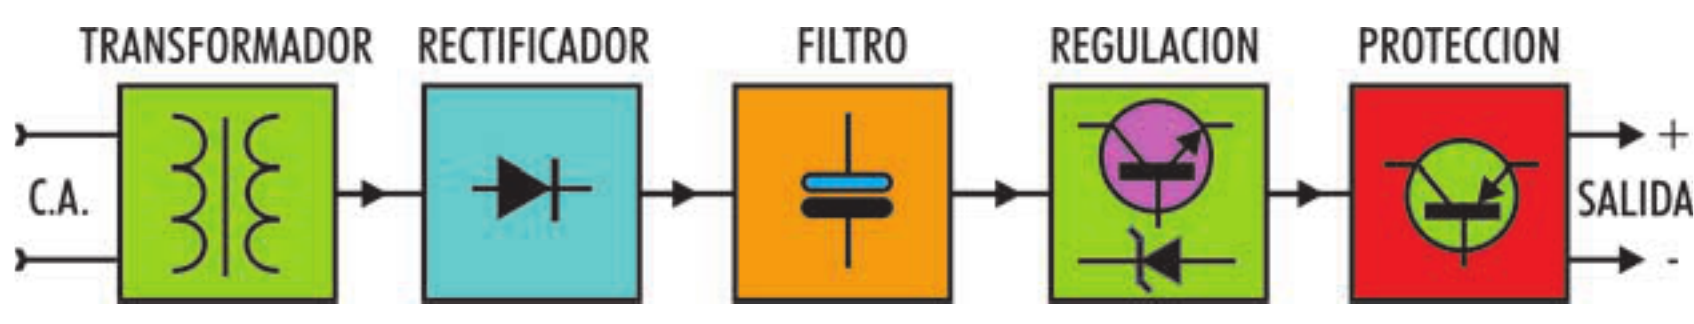
\includegraphics[width=0.82\linewidth]{bloques_fuente_es.png}
  \caption[Etapas de una fuente de alimentación DC]{Etapas de una fuente de alimentación
  DC. La de esta práctica llega hasta el bloque de regulación.}
  \label{fig:bloques}
\end{figure}

%-----------------------------------------------------------------------
\subsection{Valor eficaz y valor de pico}
%-----------------------------------------------------------------------
Una tensión alterna no vale lo mismo en todo instante, así que hace falta acordar con qué
número se la nombra. Se usan tres, y conviene no confundirlos
(figura~\ref{fig:rms}):

\begin{itemize}
  \item El \textbf{valor de pico} $V_p$ es lo máximo que alcanza la onda, medido desde el
        cero. Es la tensión que de verdad soportan los componentes, y por eso es la que
        manda a la hora de elegirlos.
  \item El \textbf{valor pico a pico} $V_{pp}=2V_p$ es la altura total del trazo, de la
        cresta al valle.
  \item El \textbf{valor eficaz} o \textbf{rms} $V_{\text{rms}}$ es el que marca el
        multímetro cuando se mide en la escala de tensión alterna (V$\sim$), y también con
        el que se rotulan la red y los transformadores.
\end{itemize}

Para una onda senoidal, y solo para ella, los tres están ligados por
\begin{equation}
  V_p=\sqrt{2}\,V_{\text{rms}}\approx 1{,}414\,V_{\text{rms}}
  \qquad
  V_{\text{rms}}=\frac{V_p}{\sqrt{2}}\approx 0{,}707\,V_p
  \qquad
  V_{pp}=2V_p
  \label{eq:rms}
\end{equation}

Como ejemplo, apliquemos las tres relaciones a la red peruana, cuyos \qty{220}{\volt} de
rótulo son un valor eficaz:
\[
  V_p=1{,}414\times\qty{220}{\volt}=\qty{311}{\volt}
  \qquad
  V_{pp}=2\times\qty{311}{\volt}=\qty{622}{\volt}
\]

\begin{figure}[H]
  \centering
  \begin{tikzpicture}
  \begin{axis}[
      width=10.5cm, height=5.0cm,
      axis lines=middle, axis line style={-},
      xmin=0, xmax=6.6, ymin=-1.45, ymax=1.65,
      xtick=\empty, ytick={-1,-0.707,0.707,1},
      yticklabels={$-V_p$,,,$V_p$},
      xlabel={$t$}, xlabel style={at={(axis description cs:1,0.5)}, anchor=west},
      tick label style={font=\footnotesize}, clip=false,
  ]
  \addplot[blue!65!black, line width=1.2pt, samples=200, domain=0:6.4] {sin(deg(x))};
  % lineas de pico y de eficaz
  \addplot[gray, dashed, samples=2, domain=0:6.4] {1};
  \addplot[gray, dashed, samples=2, domain=0:6.4] {-1};
  \addplot[red!70!black, densely dotted, line width=1pt, samples=2, domain=0:6.4] {0.707};
  % Rotulos con los numeros reales de la red peruana: es lo que el alumno tiene en
  % el tomacorriente, asi que el simbolo de la izquierda y la cifra de la derecha
  % quedan enfrentados en la misma linea.
  \node[font=\footnotesize\bfseries, anchor=west] at (axis cs:0.05,1.5)
       {Red peruana: \qty{220}{\volt} eficaces};
  \node[font=\footnotesize, anchor=west] at (axis cs:6.45,1)
       {$V_p=\qty{311}{\volt}$};
  \node[red!70!black, font=\footnotesize, anchor=west] at (axis cs:6.45,0.707)
       {$V_{\text{rms}}=0{,}707\,V_p=\qty{220}{\volt}$};
  \node[font=\footnotesize, anchor=west] at (axis cs:6.45,-1)
       {$-V_p=\qty{-311}{\volt}$};
  % Flecha pico a pico. Ojo: no se puede escribir "<->" porque babel-spanish deja
  % activos los caracteres < y > para las comillas latinas y rompe la compilacion.
  \draw[{Stealth[length=2mm]}-{Stealth[length=2mm]}, black, line width=0.8pt]
       (axis cs:1.571,1) -- (axis cs:1.571,-1);
  \node[fill=white, inner sep=1pt, font=\footnotesize] at (axis cs:1.571,0.28)
       {$V_{pp}=\qty{622}{\volt}$};
  \end{axis}
  \end{tikzpicture}
  \caption[Valor de pico, pico a pico y eficaz]{Los tres valores de una senoide, rotulados
  con los números de la red peruana. El bobinado secundario del transformador se lee igual: los
  \qty{24}{\volt} que marca el multímetro son \qty{33.9}{\volt} de pico y
  \qty{67.9}{\volt} de pico a pico. Esos \qty{311}{\volt} explican por qué el
  osciloscopio nunca se conecta al bobinado primario.}
  \label{fig:rms}
\end{figure}

%-----------------------------------------------------------------------
\subsection{Transformador}
%-----------------------------------------------------------------------
Esta etapa tiene como finalidad reducir los \qty{220}{\volt} de la red a los
\qty{24}{\volt} que necesita el resto del circuito y, además, aislar magnéticamente el
montaje de la línea. Consta de dos bobinados arrollados sobre un mismo núcleo de hierro:
el \textbf{bobinado primario}, que es el que se conecta a la red, y el
\textbf{bobinado secundario}, del que sale la tensión ya reducida hacia el resto del
circuito. Entre los dos no hay ningún
contacto eléctrico (la energía pasa de uno a otro por el campo magnético del núcleo), y en
eso consiste el aislamiento. Es un componente pasivo: no amplifica ni rectifica nada, solo
cambia la escala de la tensión. Su comportamiento se resume en dos ecuaciones:

\begin{enumerate}[label=\textbf{\alph*)}, leftmargin=*, labelsep=0.6em]
\item La \textbf{relación de transformación}. El transformador reduce la tensión en la
misma proporción en que el bobinado secundario tiene menos vueltas que el bobinado
primario.
\begin{equation}
  \frac{V_{\text{sec}}}{V_{\text{pri}}}=\frac{N_{\text{sec}}}{N_{\text{pri}}}
  \label{eq:transformacion}
\end{equation}
donde $V_{\text{pri}}$ y $V_{\text{sec}}$ son las tensiones eficaces del bobinado primario y
del bobinado secundario, y $N_{\text{pri}}$ y $N_{\text{sec}}$ el número de vueltas de cada
uno. En nuestro transformador la proporción es $24/220\approx 1/9$: el bobinado secundario
tiene unas nueve veces menos vueltas que el bobinado primario.

\item El \textbf{paso de valor eficaz a valor de pico}. El transformador viene rotulado
como \qty{24}{\volt}, pero ese número no es la tensión máxima que entrega: es su
\emph{valor eficaz}, que es el que marca el multímetro. La tensión del bobinado secundario
no vale lo mismo en todo instante, sino que oscila, y en cada ciclo llega a un máximo
bastante más alto que el del rótulo. Ese máximo es el \textbf{valor de pico}, y es el que
ven de verdad los diodos y el condensador. Se obtiene multiplicando el valor eficaz
por $\sqrt{2}$:
\begin{equation}
  V_{p(\text{sec})}=\sqrt{2}\,V_{\text{rms}}=1{,}414\times\qty{24}{\volt}=\qty{33.9}{\volt}
  \label{eq:pico-sec}
\end{equation}
Dicho de otro modo: un transformador rotulado como \qty{24}{\volt} entrega en realidad
picos de casi \qty{34}{\volt}, un \qty{41}{\percent} más. Estos \qty{33.9}{\volt} son el
punto de partida de todos los cálculos de las etapas siguientes.
\end{enumerate}

\begin{notatec}{por qué esto decide los componentes}
El transformador dice \qty{24}{\volt} porque ese es su valor eficaz, $V_{\text{rms}}$,
pero el condensador se carga hasta el \textbf{pico}, $V_{p(\text{sec})}=\qty{33.9}{\volt}$
por la ecuación~\eqref{eq:pico-sec}. Si eligiera C1 pensando en los \qty{24}{\volt} del
rótulo, se quedaría corto. Lo mismo pasa con la tensión inversa que aguantan los diodos:
también se calcula sobre $V_{p(\text{sec})}$, nunca sobre $V_{\text{rms}}$.
\end{notatec}

%-----------------------------------------------------------------------
\subsection{Rectificador}
%-----------------------------------------------------------------------
Esta etapa tiene como finalidad rectificar el semiciclo negativo de la señal alterna que
entrega el bobinado secundario, de modo que se aprovechen los dos semiciclos de la onda y
no solo uno. En esta fuente se resuelve con un \textbf{puente rectificador}: un conjunto
de cuatro diodos conectados en puente, encapsulados en un solo componente.

Lo consigue porque los diodos conducen por parejas, según hacia dónde apunte la tensión
del bobinado secundario en cada instante. En el semiciclo positivo conducen $D_1$ y $D_2$;
en el negativo, $D_3$ y $D_4$. Las dos parejas están dispuestas de modo que la corriente
atraviesa la carga siempre en el mismo sentido (figura~\ref{fig:puente}), así que el
semiciclo negativo no se descarta: se invierte y se aprovecha. De ahí que la ondulación
salga al doble de la frecuencia de red, \qty{120}{\hertz}.

Ese aprovechamiento tiene un precio. En cada semiciclo la corriente atraviesa dos diodos
en serie con la carga, y cada uno cae unos \qty{0.7}{\volt}, de manera que el pico a la
salida del puente queda \qty{1.4}{\volt} por debajo del pico del bobinado secundario:
\begin{equation}
  V_{p(\text{out})}=V_{p(\text{sec})}-\qty{1.4}{\volt}
  \label{eq:vpout}
\end{equation}
Con los \qty{33.9}{\volt} de pico que entrega nuestro bobinado secundario, a la salida del
puente quedan \qty{32.5}{\volt}.

\begin{figure}[H]
  \centering
  \begin{subfigure}{0.49\linewidth}
    \centering
    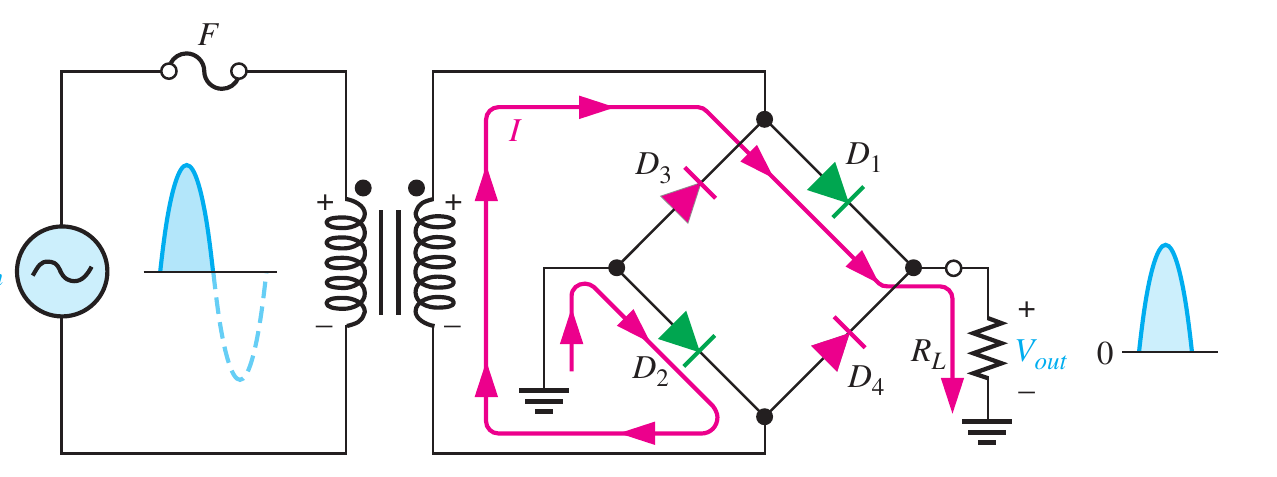
\includegraphics[width=\linewidth]{puente_semiciclo_pos.png}
    \caption{Semiciclo positivo: conducen $D_1$ y $D_2$.}
  \end{subfigure}\hfill
  \begin{subfigure}{0.49\linewidth}
    \centering
    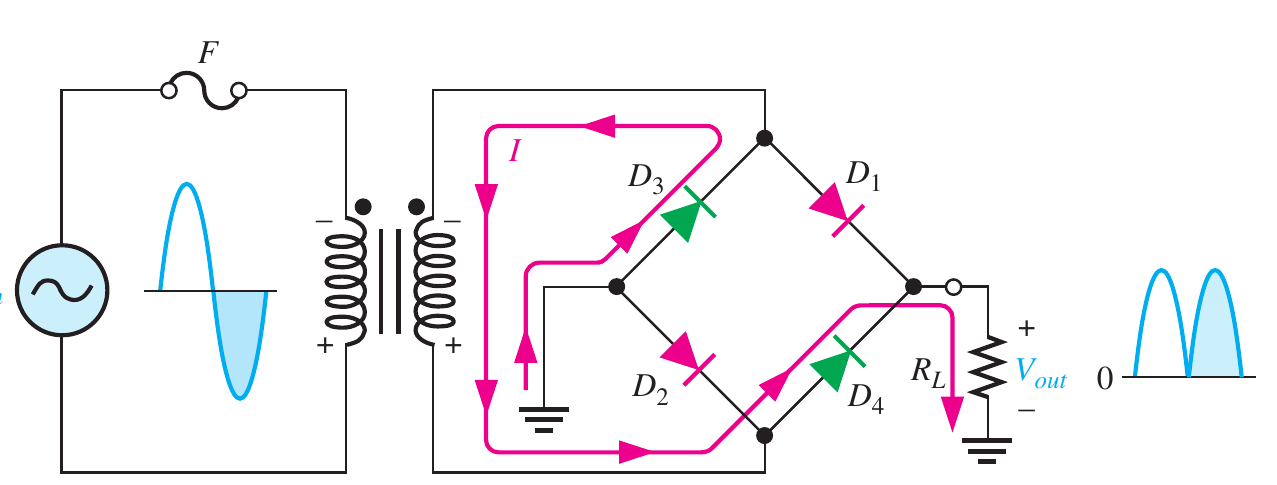
\includegraphics[width=\linewidth]{puente_semiciclo_neg.png}
    \caption{Semiciclo negativo: conducen $D_3$ y $D_4$.}
  \end{subfigure}
  \caption[Funcionamiento del puente rectificador]{Funcionamiento del puente
  rectificador: en los dos semiciclos la corriente recorre $R_L$ en el mismo sentido.}
  \label{fig:puente}
\end{figure}
%-----------------------------------------------------------------------
\subsection{Filtro}
%-----------------------------------------------------------------------
Esta etapa tiene como finalidad alisar la tensión que sale del puente, que es continua
pero pulsante: oscila 120 veces por segundo. Para conseguirlo se conecta un
condensador en paralelo con la salida, y este trabaja en dos tiempos. Mientras la señal
rectificada sube, el condensador \textbf{se carga} hasta alcanzar el valor de pico.
Cuando la señal empieza a bajar, el condensador \textbf{se descarga} poco a poco sobre lo
que tiene conectado a continuación (en esta fuente, el regulador y lo que se enchufe a su
salida) y sostiene la tensión hasta que llega el pico siguiente, de manera
que ya no cae hasta cero (figura~\ref{fig:rizado-partes}). Lo que queda es una tensión
continua con una ondulación montada encima, y a esa ondulación se le llama \emph{rizado} ($V_r$).
Para describir esa señal hacen falta dos números:

\begin{figure}[H]
  \centering
  % Figura propia, no sale de ningun libro: los esquemas de Floyd dibujan el rizado
  % pero no rotulan V_r(pp) ni V_DC, que es justo lo que el alumno necesita ver para
  % entender las ecuaciones (5) a (7). El rizado va exagerado (aqui ~32 %, en la
  % fuente real mucho menos): a escala real las tres lineas quedarian superpuestas.
  % Geometria: picos en x = 1, 3, 5 y 7; el valle se fija en 0,62 y la sinusoide
  % vuelve a alcanzar ese valor en x = 2,4257, que es donde termina cada descarga.
  \begin{tikzpicture}[x=1.35cm, y=3.0cm, line cap=round]
    % --- niveles de referencia
    \draw[gray!60, dashed] (0,1)    -- (7.5,1);
    \draw[gray!60, dashed] (0,0.62) -- (7.5,0.62);
    \draw[red!70!black, line width=0.9pt] (0,0.81) -- (7.5,0.81);
    % --- senal rectificada, tal como sale del puente (sin condensador)
    \draw[gray!55, dashed, line width=0.8pt, samples=300, domain=0:7.3]
         plot (\x, {abs(sin(90*\x))});
    % --- tension en el condensador: se recarga siguiendo la sinusoide y se
    %     descarga en linea recta sobre lo que tenga conectado
    \draw[blue!65!black, line width=1.3pt, samples=60, domain=0:1]
         plot (\x, {abs(sin(90*\x))});
    \draw[blue!65!black, line width=1.3pt] (1,1) -- (2.4257,0.62);
    \draw[blue!65!black, line width=1.3pt, samples=40, domain=2.4257:3]
         plot (\x, {abs(sin(90*\x))});
    \draw[blue!65!black, line width=1.3pt] (3,1) -- (4.4257,0.62);
    \draw[blue!65!black, line width=1.3pt, samples=40, domain=4.4257:5]
         plot (\x, {abs(sin(90*\x))});
    \draw[blue!65!black, line width=1.3pt] (5,1) -- (6.4257,0.62);
    \draw[blue!65!black, line width=1.3pt, samples=40, domain=6.4257:7]
         plot (\x, {abs(sin(90*\x))});
    % --- que es el rizado: la propia ondulacion, senalada sobre la onda
    \node[font=\footnotesize, anchor=west, inner sep=2pt] (rz) at (1.30,0.28)
         {el \textbf{rizado} es esta ondulación};
    \draw[-{Stealth[length=1.8mm]}, gray!35!black, line width=0.7pt]
         (rz.north east) to[bend left=14] (4.35,0.66);
    % --- ejes
    \draw[-{Stealth[length=2mm]}] (0,0) -- (8.0,0)
         node[anchor=west, font=\footnotesize] {$t$};
    \draw[-{Stealth[length=2mm]}] (0,0) -- (0,1.32);
    \node[font=\footnotesize, anchor=north east] at (0,0) {0};
    % --- rotulos de las tres magnitudes
    \node[font=\footnotesize, anchor=east] at (-0.12,1) {$V_{p(\text{rect})}$};
    \node[red!70!black, font=\footnotesize, anchor=east] at (-0.12,0.81)
         {$V_{\text{DC}}$};
    \draw[{Stealth[length=2mm]}-{Stealth[length=2mm]}, line width=0.8pt]
         (7.35,0.62) -- (7.35,1);
    \node[font=\footnotesize, anchor=west, inner sep=2pt] at (7.52,0.81)
         {$V_{r(pp)}$};
    % --- leyenda
    \draw[blue!65!black, line width=1.3pt] (0.15,1.2) -- (0.60,1.2);
    \node[font=\footnotesize, anchor=west] at (0.68,1.2) {tensión en C1, con filtro};
    \draw[gray!55, dashed, line width=0.8pt] (3.50,1.2) -- (3.95,1.2);
    \node[font=\footnotesize, anchor=west] at (4.03,1.2)
         {salida del puente, sin filtro};
  \end{tikzpicture}
  \caption[Las tres magnitudes del filtro]{Las tres magnitudes de las
  ecuaciones~\eqref{eq:rizado} a~\eqref{eq:factor-rizado} sobre la forma de onda. El rizado
  va dibujado exagerado para que se distingan las tres líneas.}
  \label{fig:rizado-partes}
\end{figure}

\begin{enumerate}[label=\textbf{\alph*)}, leftmargin=*, labelsep=0.6em]
\item La \textbf{tensión de rizado} $V_{r(pp)}$: la altura de la ondulación, medida de su
punto más bajo al más alto. Es decir, el valor pico a pico de lo que le sobra a la
continua; de ahí el subíndice $pp$. Es lo que se lee en el osciloscopio con acoplamiento
AC:
\begin{equation}
  V_{r(pp)}\approx\left(\frac{1}{f\,R_L\,C_1}\right)V_{p(\text{rect})}
  \label{eq:rizado}
\end{equation}

\item La \textbf{tensión continua} $V_{\text{DC}}$: el valor medio de esa misma señal, la
altura alrededor de la cual ondula. Es lo que marca el multímetro en continua, y es la
tensión que realmente le llega al regulador:
\begin{equation}
  V_{\text{DC}}\approx\left(1-\frac{1}{2f\,R_L\,C_1}\right)V_{p(\text{rect})}
  \label{eq:vdc}
\end{equation}
\end{enumerate}

En las dos, $V_{p(\text{rect})}$ es el pico de la señal rectificada que entra al filtro, el
de la ecuación~\eqref{eq:vpout}; $f=\qty{120}{\hertz}$ es la frecuencia del rizado, que en
un puente es el doble de la de red; $C_1$ es la capacidad del condensador de filtro y $R_L$
la resistencia de carga (figura~\ref{fig:rl}).

\begin{figure}[H]
  \centering
  % Esquema propio. Responde a una pregunta que la guia dejaba en el aire: de donde
  % sale la R_L de las ecuaciones (5) y (6) si en el circuito no hay ninguna
  % resistencia de carga montada.
  \begin{subfigure}{0.48\linewidth}
    \centering
    \begin{tikzpicture}[x=0.6cm, y=0.6cm, line width=0.8pt, line cap=round]
      \draw (0.4,2.6) -- (9.6,2.6);
      \draw (0.4,0)   -- (9.6,0);
      \draw[fill=white] (0.4,2.6) circle (0.16);
      \draw[fill=white] (0.4,0)   circle (0.16);
      \node[font=\scriptsize, anchor=west] at (0.15,3.2) {del puente};
      % condensador de filtro
      \draw (3.6,2.6) -- (3.6,1.55);
      \draw (2.9,1.55) -- (4.3,1.55);
      \draw (2.9,1.25) -- (4.3,1.25);
      \draw (3.6,1.25) -- (3.6,0);
      \node[font=\scriptsize, anchor=west] at (4.45,1.4) {C1};
      % resistencia de carga
      \draw (7.6,2.6) -- (7.6,1.85);
      \draw[fill=white] (7.2,1.85) rectangle (8.0,0.75);
      \draw (7.6,0.75) -- (7.6,0);
      \node[font=\scriptsize, anchor=west] at (8.15,1.3) {$R_L$};
      \fill (3.6,2.6) circle (0.1); \fill (3.6,0) circle (0.1);
      \fill (7.6,2.6) circle (0.1); \fill (7.6,0) circle (0.1);
    \end{tikzpicture}
    \caption{Como lo dibujan los libros.}
  \end{subfigure}\hfill
  \begin{subfigure}{0.48\linewidth}
    \centering
    \begin{tikzpicture}[x=0.6cm, y=0.6cm, line width=0.8pt, line cap=round]
      \draw (0.4,2.6) -- (10.2,2.6);
      \draw (0.4,0)   -- (10.2,0);
      \draw[fill=white] (0.4,2.6) circle (0.16);
      \draw[fill=white] (0.4,0)   circle (0.16);
      \node[font=\scriptsize, anchor=west] at (0.15,3.2) {del puente};
      % condensador de filtro
      \draw (3.0,2.6) -- (3.0,1.55);
      \draw (2.3,1.55) -- (3.7,1.55);
      \draw (2.3,1.25) -- (3.7,1.25);
      \draw (3.0,1.25) -- (3.0,0);
      \node[font=\scriptsize, anchor=east] at (2.15,1.4) {C1};
      % lo que hay de verdad
      \draw[gray!60, dashed, line width=0.7pt] (4.6,0.3) rectangle (8.9,2.3);
      \draw (6.75,2.6) -- (6.75,2.05);
      \draw[fill=black!5] (5.1,2.05) rectangle (8.4,0.55);
      \node[font=\scriptsize] at (6.75,1.55) {regulador};
      \node[font=\scriptsize] at (6.75,1.05) {y carga};
      \draw (6.75,0.55) -- (6.75,0);
      \node[font=\scriptsize, fill=white, inner sep=1pt] at (4.6,2.3) {$R_L$};
      \fill (6.75,2.6) circle (0.1); \fill (6.75,0) circle (0.1);
      \fill (3.0,2.6) circle (0.1); \fill (3.0,0) circle (0.1);
    \end{tikzpicture}
    \caption{Lo que hay en esta fuente.}
  \end{subfigure}
  \caption[De dónde sale la $R_L$ de las ecuaciones]{De dónde sale la $R_L$ de las
  ecuaciones~\eqref{eq:rizado} y~\eqref{eq:vdc}. Los libros dibujan a la salida del filtro
  una resistencia de carga; en esta fuente no hay ninguna, porque lo que C1 alimenta es el
  regulador y lo que se conecte a su salida. $R_L$ es el modelo de ese consumo: la
  resistencia que absorbería la misma corriente, $R_L=V_{\text{DC}}/I$.}
  \label{fig:rl}
\end{figure}

Las dos cifras se combinan en una sola medida de calidad, el \textbf{factor de rizado} $r$,
que compara lo que ondula con lo que vale la continua:
\begin{equation}
  r=\frac{V_{r(pp)}}{V_{\text{DC}}}
  \label{eq:factor-rizado}
\end{equation}
Como es un cociente entre dos tensiones, $r$ no tiene unidades y se suele expresar en
porcentaje: cuanto más pequeño, más se parece la salida a una continua ideal. En las dos
ecuaciones anteriores $C_1$ y $R_L$ aparecen dividiendo, así que aumentar cualquiera de los
dos reduce $V_{r(pp)}$, sube $V_{\text{DC}}$ y por tanto mejora $r$ (figura~\ref{fig:rizado}).

\begin{figure}[H]
  \centering
  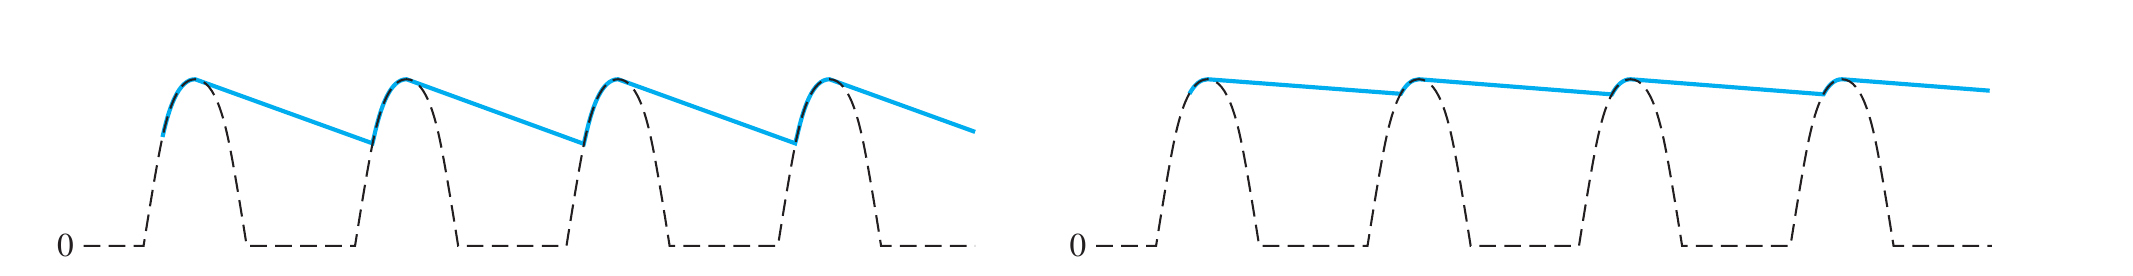
\includegraphics[width=0.88\linewidth]{rizado_filtro.png}
  \caption[Rizado a la salida del filtro]{Rizado (línea continua) sobre la señal
  rectificada (línea de trazos). A la derecha, el mismo circuito con más capacidad.}
  \label{fig:rizado}
\end{figure}

% Ejemplo resuelto con los valores de ESTA fuente. Va aqui a proposito: el
% alumno de tercer semestre no ha visto rizado antes, y con un caso numerico
% delante repite el patron en la seccion VI sin tener que despejar nada.
\begin{ejemplo}{el rizado de nuestra fuente con una carga de \qty{100}{\ohm}}
Partimos del bobinado secundario, \qty{24}{\volt} eficaces, con
$C_1=\qty{2200}{\micro\farad}$ y $f=\qty{120}{\hertz}$. El pico del bobinado secundario y el
de la señal rectificada son
\[
  V_{p(\text{sec})}=1{,}414\times\qty{24}{\volt}=\qty{33.9}{\volt}
  \qquad
  V_{p(\text{rect})}=\qty{33.9}{\volt}-\qty{1.4}{\volt}=\qty{32.5}{\volt}
\]
Sustituyendo en las ecuaciones~\eqref{eq:rizado} y~\eqref{eq:vdc}, con
$R_L=\qty{100}{\ohm}$:
\[
  V_{r(pp)}\approx\frac{\qty{32.5}{\volt}}{120\times100\times2200\times10^{-6}}
  =\frac{\qty{32.5}{\volt}}{26{,}4}=\qty{1.23}{\volt}
\]
\[
  V_{\text{DC}}\approx\left(1-\frac{1}{2\times120\times100\times2200\times10^{-6}}\right)
  \qty{32.5}{\volt}=0{,}981\times\qty{32.5}{\volt}=\qty{31.9}{\volt}
\]
El factor de rizado resulta $r=\qty{1.23}{\volt}/\qty{31.9}{\volt}=0{,}039$, es decir un
\qty{3.9}{\percent}.
\end{ejemplo}

%-----------------------------------------------------------------------
\subsection{Regulador}
%-----------------------------------------------------------------------
Esta etapa tiene como finalidad fijar el voltaje de salida en el valor elegido y
sostenerlo ahí, absorbiendo las variaciones que le llegan por delante. Hace falta porque
el filtro entrega una tensión continua, pero no \emph{estable}: su valor oscila con la
red y, sobre todo, se hunde en cuanto la carga pide más corriente.

El regulador usado en esta fuente es un LM317, que no entrega una tensión fija sino
\textbf{ajustable}: su tensión de salida no viene impuesta por el integrado, sino que la
fijan dos resistencias conectadas por fuera, R1 y el potenciómetro RV1. Girando RV1 se
elige la tensión que entrega la fuente.
Todo su funcionamiento se resume en una sola propiedad, y conviene retenerla
porque de ella sale el resto: \textbf{el integrado hace lo que haga falta para mantener
siempre \qty{1.25}{\volt} entre su terminal de salida (V\textsubscript{OUT}) y su terminal
de ajuste (ADJ)}. A esa tensión se le llama tensión de referencia.

\begin{figure}[H]
  \centering
  % Recorte de la etapa de regulacion tomado tal cual del esquema completo de la
  % figura 8, sin redibujar nada: asi el alumno ve exactamente el mismo dibujo que
  % va a montar, en lugar de dos representaciones distintas del mismo circuito.
  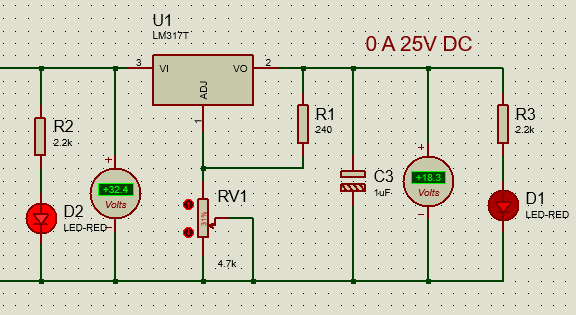
\includegraphics[width=0.55\linewidth]{regulador_recorte.png}
  \caption[La etapa de regulación]{La etapa de regulación, recortada del circuito
  completo de la figura~\ref{fig:circuito}. En el esquema, VI y VO son los terminales
  V\textsubscript{IN} y V\textsubscript{OUT} del LM317.}
  \label{fig:regulador}
\end{figure}

Esa propiedad es la que convierte a $R_1$ y $R_{V1}$ en el mando de la fuente
(figura~\ref{fig:regulador}). Como sobre
$R_1$ hay \qty{1.25}{\volt} fijos, por ella circula una corriente que no depende del ajuste:
\[
  I=\frac{\qty{1.25}{\volt}}{R_1}=\frac{\qty{1.25}{\volt}}{\qty{240}{\ohm}}
   =\qty{5.2}{\milli\ampere}
\]
Esa misma corriente continúa por $R_{V1}$, porque la que se va por el terminal ADJ es
despreciable (unos \qty{50}{\micro\ampere}). Sobre $R_{V1}$ aparece entonces una caída
$I\,R_{V1}$, y la salida es la suma de las dos caídas:
\begin{equation}
  V_{\text{OUT}}=\qty{1.25}{\volt}\left(1+\frac{R_{V1}}{R_1}\right)
  \label{eq:lm317}
\end{equation}
En esa expresión se lee el rango de ajuste de la fuente. Con $R_{V1}=0$ la salida vale
\qty{1.25}{\volt}, que es el mínimo; con $R_{V1}$ al máximo, \qty{4.7}{\kilo\ohm}, sube
hasta $\qty{1.25}{\volt}\,(1+4700/240)=\qty{25.7}{\volt}$, los \qty{26}{\volt} que da la
simulación.

Por último, la calidad de un regulador se mide con dos cifras:

\begin{enumerate}[label=\textbf{\alph*)}, leftmargin=*, labelsep=0.6em]
\item La \textbf{regulación de línea} dice cuánto se mueve la tensión de salida cuando se
mueve la de entrada. Mide si el regulador aguanta las subidas y bajadas de la red:
\begin{equation}
  \text{Regulación de línea}=\left(\frac{\Delta V_{\text{OUT}}}{\Delta V_{\text{IN}}}\right)100\%
\end{equation}
donde $\Delta V_{\text{IN}}$ es lo que varía la tensión de entrada y $\Delta V_{\text{OUT}}$
lo que varía la de salida por causa de ello.

\item La \textbf{regulación de carga} dice cuánto se mueve la tensión de salida cuando
cambia la corriente que se le pide. Mide si la fuente se hunde al conectarle una carga:
\begin{equation}
  \text{Regulación de carga}=\left(\frac{V_{\text{NL}}-V_{\text{FL}}}{V_{\text{FL}}}\right)100\%
\end{equation}
donde $V_{\text{NL}}$ es la tensión de salida sin carga y $V_{\text{FL}}$ la que queda a
plena carga.
\end{enumerate}

En las dos, cuanto más pequeño sea el resultado, mejor es el regulador: quiere decir que la
salida apenas se entera de lo que cambia a su alrededor.

\FloatBarrier
%=======================================================================
\section{Circuito propuesto}
%=======================================================================
La figura~\ref{fig:circuito} es el circuito que se va a montar, con las tensiones que
entrega la simulación. El transformador TR1 baja los \qty{220}{\volt} de la red a
\qty{24}{\volt}; el puente BR1 los rectifica y C1 los filtra, con lo que a la entrada del
regulador hay \qty{32.6}{\volt} de continua. El regulador es un LM317, que no da una
tensión fija sino ajustable: R1 y el potenciómetro RV1 fijan la salida según la
ecuación~\eqref{eq:lm317} del marco teórico.
Con $R_1=\qty{240}{\ohm}$ y RV1 al máximo la salida llega a los \qty{26}{\volt} de la
simulación, y con RV1 a cero baja hasta \qty{1.25}{\volt}: ese es el rango de ajuste de la
fuente.

\begin{figure}[H]
  \centering
  % Version con los dos LED indicadores. No lleva los recuadros de etapa que tenia la
  % version anterior: el propio esquema ya trae rotulo y rango, y las cajas se
  % solapaban con ese texto.
  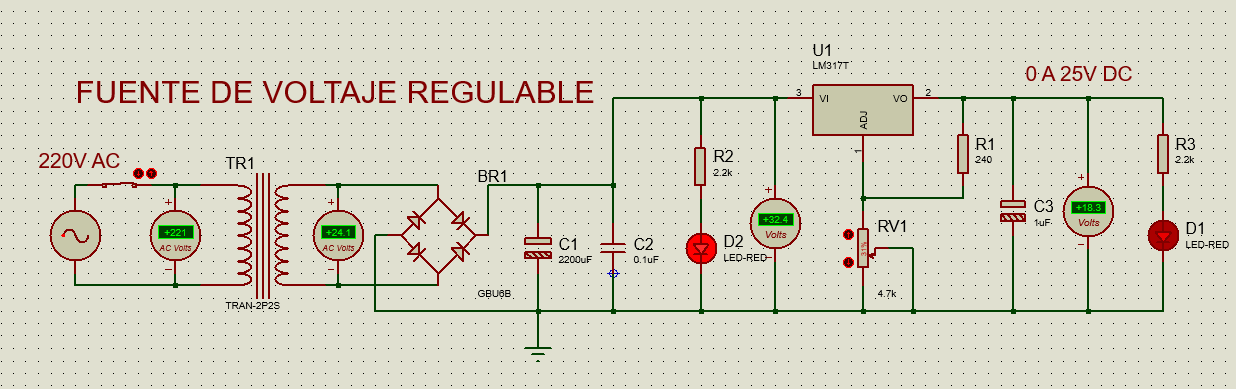
\includegraphics[width=\linewidth]{fuente.png}
  \caption[Circuito de la fuente DC ajustable]{Circuito de la fuente, simulado en Proteus.
  Se recorre de izquierda a derecha en cuatro etapas: transformador (TR1), rectificador
  (BR1), filtro (C1 y C2) y regulador (U1, R1 y RV1). D2 indica que hay tensión a la
  entrada del regulador y D1 que la hay a la salida. El interruptor de red no aparece en el
  esquema: va en serie con el bobinado primario de TR1, antes del transformador.}
  \label{fig:circuito}
\end{figure}

\FloatBarrier
%=======================================================================
\section{Equipos y materiales}
%=======================================================================
\noindent\textbf{Equipos y dispositivos:}
\begin{itemize}
    \item Osciloscopio Tektronix.
    \item 02 puntas de osciloscopio.
    \item Multímetro.
\end{itemize}

\begin{notatec}{la red no se mide con una punta normal}
El osciloscopio sí puede medir \qty{220}{\volt}, pero no con las puntas habituales: su
pinza de masa está unida a la tierra de la red por el propio enchufe del equipo, así que
sujetarla a un conductor de la red lo cortocircuita contra tierra. Para medir ahí harían
falta una \textbf{punta diferencial} o un \textbf{transformador de aislamiento}, que no se
usan en esta práctica.
\begin{itemize}
    \item Con el material de esta práctica, \textbf{no} conecte el osciloscopio al bobinado
          primario ni a ningún punto de la red.
    \item Del bobinado secundario en adelante todo es baja tensión y se mide con
          normalidad, llevando siempre la pinza de masa al negativo del montaje.
\end{itemize}
\end{notatec}

\noindent\textbf{Software:}
\begin{itemize}
    \item Simulador de circuitos: Proteus o Multisim.
\end{itemize}

\vspace{0.25cm}
\noindent\textbf{Materiales y fungibles} (deben ser adquiridos por los alumnos). Los
componentes que pueden quemarse en el montaje van \textbf{por duplicado}: son baratos y
así una avería no deja el laboratorio a medias.
\begin{itemize}
    % --- Etapa de red y transformador. Ni el transformador ni el interruptor se
    % duplican: son los dos componentes caros y no estan en el camino de la averia.
    \item 01 transformador de \qty{220}{\volt} a \qty{24}{\volt}, de \qty{2}{\ampere}
          (TR1).
    % El alumno olvido dibujarlo en el esquema; va en el primario, antes de TR1.
    \item 01 interruptor de red para \qty{220}{\volt}, de 2 a \qty{3}{\ampere}.
    \item 01 cable de alimentación con enchufe.
    % --- Rectificacion. El GBU6B es de 6 A y 100 V; la PIV que exige el circuito es
    % de solo 33,4 V, asi que va sobrado. Aun asi se duplica: un corto a la salida o
    % un electrolitico al reves se lo llevan por delante.
    \item \textbf{02} puentes rectificadores GBU6B (\qty{6}{\ampere}, \qty{100}{\volt})
          (BR1).
    % --- Filtro. C1 ve los 32,6 V de pico: la regla practica pide un condensador de
    % al menos un 50 % mas, y el valor normalizado que sigue es 50 V.
    % Los electroliticos son polarizados: montarlos al reves es el error clasico y
    % terminan reventando. Por eso van dobles.
    \item \textbf{02} condensadores electrolíticos de \qty{2200}{\micro\farad} /
          \qty{50}{\volt} (C1).
    \item \textbf{02} condensadores cerámicos de \qty{0.1}{\micro\farad} /
          \qty{50}{\volt} (C2).
    \item \textbf{02} condensadores electrolíticos de \qty{1}{\micro\farad} /
          \qty{50}{\volt} (C3).
    % --- Regulacion. El LM317 es el que mas se quema: se lleva toda la diferencia
    % entre la entrada y la salida en forma de calor.
    \item \textbf{02} reguladores LM317T (U1).
    % Por R1 y RV1 circulan 5,2 mA: disipan milivatios, de ahi el 1/4 W. Se duplican
    % porque si cualquiera de los dos se abre, la salida salta al maximo y arrastra
    % a lo que este conectado.
    \item \textbf{02} resistencias de \qty{240}{\ohm} (1/4\,\unit{\watt}) (R1).
    \item \textbf{02} potenciómetros de \qty{4.7}{\kilo\ohm} (RV1).
    % El LM317 se lleva la diferencia entre sus 32,6 V de entrada y la salida: en el
    % extremo bajo del ajuste eso son decenas de vatios. Sin disipador no aguanta.
    \item 01 disipador para el LM317T, con su tornillo y su mica aislante.
    % --- Indicadores. D2 avisa de que hay tension a la entrada del regulador y D1
    % de que la hay a la salida. R2 ve los 32,4 V del filtro: descontando los 2 V del
    % LED circulan 13,8 mA y disipa 0,42 W, de ahi el vatio y no 1/4 W. En R3, con la
    % salida en 25 V, son 10,5 mA y 0,24 W. Los LED van dobles: montados al reves no
    % encienden y es el error tipico.
    \item \textbf{04} diodos LED rojos (D1 y D2, dos de repuesto).
    \item \textbf{04} resistencias de \qty{2.2}{\kilo\ohm} (1\,\unit{\watt}) (R2 y R3,
          dos de repuesto).
    % --- Montaje. Se arma en protoboard, pero el primario NO: ver la caja de
    % seguridad. De ahi la bornera y el aislante, que son solo para ese tramo.
    \item 01 protoboard.
    \item Cables conectores para protoboard.
    \item 01 bornera de conexión y cinta aislante o tubo termorretráctil, para cablear
          el bobinado primario fuera del protoboard.
    \item Mandil (obligatorio).
\end{itemize}

\begin{seguridad}{el bobinado primario no va en el protoboard}
La fuente se arma en protoboard \textbf{a partir del bobinado secundario}. El tramo enchufe --
interruptor -- bobinado primario de TR1 está a \qty{220}{\volt} y sus contactos quedarían
accesibles: cablee ese tramo aparte, con bornera y las uniones aisladas, y déjelo
desconectado mientras trabaja. Desde el bobinado secundario en adelante todo es baja tensión y se
maneja con normalidad, siempre con la fuente desenchufada.
\end{seguridad}

\FloatBarrier
%=======================================================================
\section{Construcción}
%=======================================================================
El montaje se hace \textbf{en clase} y sobre \textbf{protoboard}, salvo el bobinado
primario. La fuente se arma \textbf{etapa por etapa} siguiendo el circuito propuesto de la
figura~\ref{fig:circuito}: primero el transformador, después el rectificador, luego el filtro
y por último el regulador. No pase a la siguiente etapa hasta que la anterior entregue la
tensión que le corresponde. Al terminar cada una, mida y capture la señal con el
osciloscopio y anote el resultado en la tabla~\ref{tab:puesta-marcha}. La figura~\ref{fig:armado} sirve de
referencia para el cableado de las tres primeras etapas.

\begin{figure}[H]
  \centering
  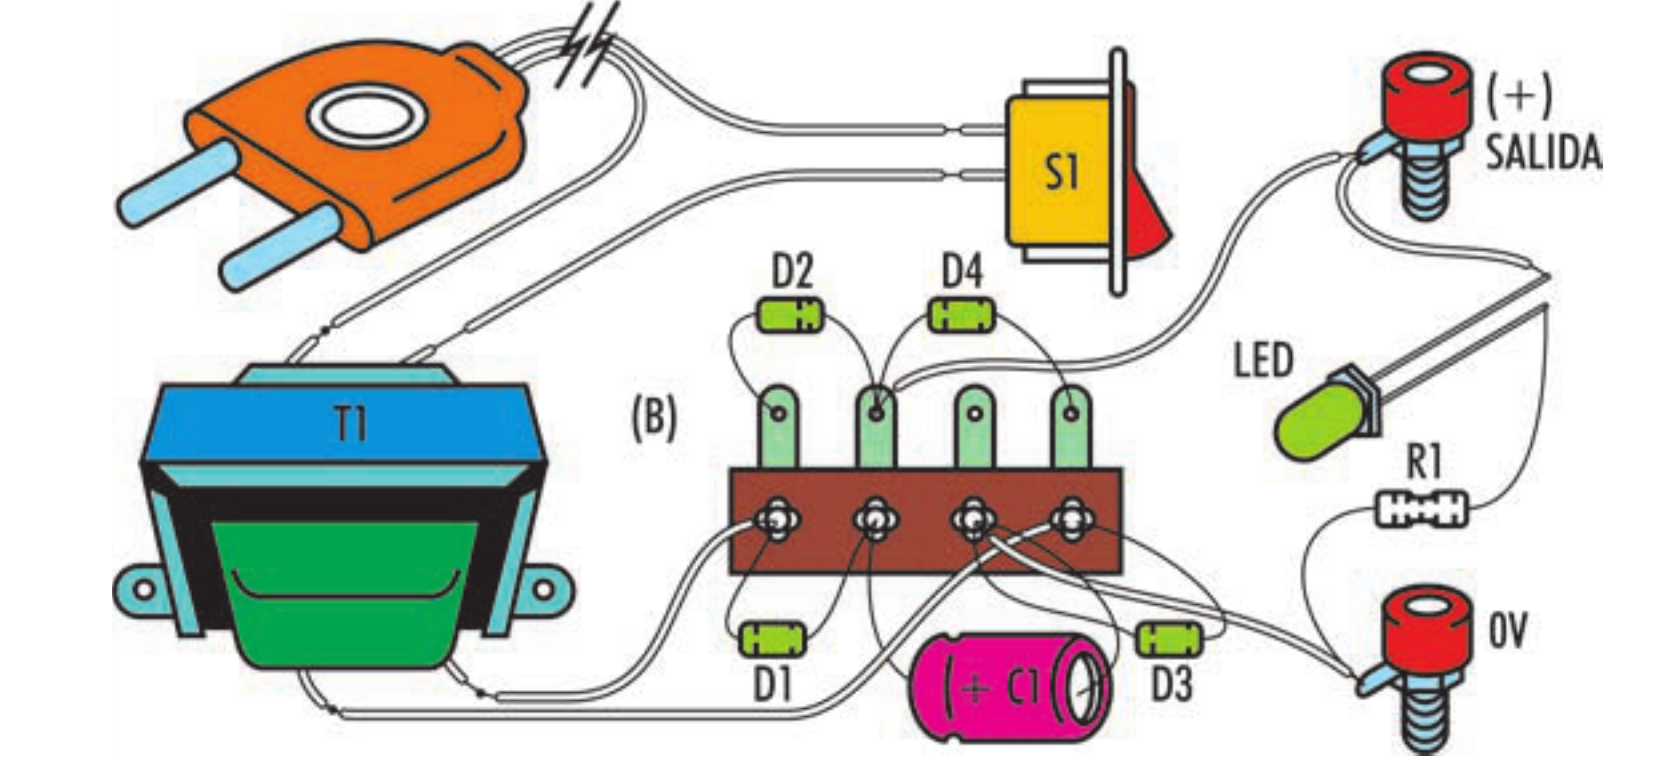
\includegraphics[width=0.78\linewidth]{armado_puente_terminales.png}
  \caption[Cableado de las tres primeras etapas]{Cableado de las tres primeras etapas, que
  son iguales a las de nuestra fuente. El folleto lo resuelve sobre un puente de
  terminales; nosotros haremos lo mismo en protoboard, con una salvedad: el tramo enchufe
  -- interruptor -- bobinado primario va cableado aparte. Tomado del folleto de Saber
  Electrónica.}
  \label{fig:armado}
\end{figure}

\begin{table}[H]
  \centering
  \caption[Puesta en marcha por etapas]{Puesta en marcha por etapas. La columna
  \textbf{Medido} no se rellena con un número suelto: cada casilla debe respaldarse con
  la \textbf{captura del osciloscopio} de esa medida, numerada y adjunta en el informe.}
  \label{tab:puesta-marcha}
  \small
  % Filas altas: el alumno tiene que poder anotar a mano en cada casilla.
  \renewcommand{\arraystretch}{2.3}
  \begin{tabularx}{\linewidth}{@{}|>{\raggedright\arraybackslash}X
                                 |>{\centering\arraybackslash}m{2.5cm}
                                 |>{\centering\arraybackslash}m{2.5cm}
                                 |>{\centering\arraybackslash}m{2.5cm}|@{}}
    \hline
    \textbf{Punto de medida} & \textbf{Calculado} & \textbf{Simulado} & \textbf{Medido}\\
    \hline
    Bobinado secundario de TR1 ($V_{\text{rms}}$ y $V_p$) & & & \\ \hline
    Salida del puente, sin C1 ($V_{\text{DC}}$) & & & \\ \hline
    Salida del filtro, con C1 ($V_{\text{DC}}$) & & & \\ \hline
    Rizado a la salida del filtro ($V_{r(pp)}$) & & & \\ \hline
    Salida mínima de la fuente ($V_{\text{DC}}$) & & & \\ \hline
    Salida máxima de la fuente ($V_{\text{DC}}$) & & & \\ \hline
  \end{tabularx}
\end{table}

\begin{seguridad}{descargue C1 antes de tocar el montaje}
C1 queda cargado a más de \qty{30}{\volt} después de desconectar y no se descarga solo.
Antes de modificar el circuito, descárguelo con una resistencia y compruebe con el
multímetro que la tensión ha bajado a cero.
\end{seguridad}

\FloatBarrier
%=======================================================================
\section{Observaciones}
%=======================================================================
Las mediciones no se entregan como números escritos en una tabla, sino como
\textbf{imágenes}: la captura del osciloscopio es la evidencia de cada medida. Presente una
captura por cada punto de medida de la tabla~\ref{tab:puesta-marcha}:

\begin{enumerate}[label=\textbf{\arabic*.}, leftmargin=*, labelsep=0.6em]
  \item Tensión en el bobinado secundario de TR1.
  \item Salida del puente rectificador, todavía sin C1.
  \item Salida del filtro, ya con C1 montado.
  \item Rizado $V_{r(pp)}$ a la salida del filtro, con el osciloscopio en acoplamiento AC.
  \item Salida de la fuente ajustada a su valor mínimo.
  \item Salida de la fuente ajustada a su valor máximo.
\end{enumerate}

En cada captura utilice los \textbf{cursores o marcadores} del osciloscopio para señalar
sobre la propia traza el valor que se está midiendo: $V_p$ y $V_{pp}$ en las señales
alternas, $V_{r(pp)}$ en el rizado y el nivel de continua donde corresponda. La lectura
del cursor debe quedar visible en la imagen.

Cada imagen debe ir numerada y llevar un pie que indique a qué punto del circuito
corresponde y con qué escalas de tiempo y de tensión se tomó. Compare después cada valor
leído con el que entrega la simulación en Proteus y comente las diferencias que encuentre.

\lineasresp{5}

\FloatBarrier

%=======================================================================
\section{Cuestionario}
%=======================================================================
\begin{enumerate}[label=\textbf{\arabic*.}, leftmargin=*, labelsep=0.6em]
\item El rizado que midió está a \qty{120}{\hertz}. Si uno de los cuatro diodos del puente
se abriera, ¿a qué frecuencia pasaría y qué le ocurriría a la tensión continua? Explique
el porqué a partir de la figura~\ref{fig:puente}.
\lineasresp{3}

\item C1 vale \qty{2200}{\micro\farad} y ya filtra. ¿Para qué sirve entonces C2, de solo
\qty{0.1}{\micro\farad}?
\lineasresp{3}

\item El transformador está rotulado como \qty{24}{\volt} y el multímetro en alterna
confirma esa lectura, pero en el osciloscopio la traza del bobinado secundario llega a casi
\qty{34}{\volt}. ¿Cómo se explica que los dos instrumentos den valores distintos midiendo lo
mismo? ¿Cuál de los dos hay que usar para decidir la tensión que debe aguantar C1, y por
qué?
\lineasresp{3}
\end{enumerate}

\FloatBarrier
%=======================================================================
\section{Conclusiones}
%=======================================================================
\begin{itemize}
    \item Deberán consignar como mínimo 05 conclusiones \textbf{cualitativas} y 05
          \textbf{cuantitativas}.
\end{itemize}

\noindent\textbf{Cualitativas}
\lineasresp{10}

\noindent\textbf{Cuantitativas}
\lineasresp{10}

\end{document}
